%\documentclass[handout]{beamer}
\documentclass[ignorenonframetext]{beamer}
\usepackage{textpos}
\usepackage{graphicx}
\usepackage{pgf}
\usepackage{caption}
\usepackage{multimedia}
\usepackage{gensymb}
\usepackage{amsmath, mathrsfs}

\captionsetup[figure]{labelformat=empty}% redefines the caption setup of the figures environment in the beamer class.

\usetheme{Boadilla}
\usefonttheme{serif}
% \mode<presentation>
% {
%  \usefonttheme{serif}
% % \useoutertheme{sidebar}
% %   \logo{\includegraphics[height=1cm]{elec_logo.pdf}}
% }

\title[TART Radio Telescope Calibration]{Continuous Antenna Calibration for the
Transient Array Radio Telescope}

\author[Molteno, Scheel]{Timothy C. A. Molteno, Max Scheel}

\institute[Otago]
{
  Elec Research \\
  Department of Physics\\
  University of Otago \\
  Dunedin, New Zealand.\\
  tim@elec.ac.nz
}

% \titlegraphic{\includegraphics[width=2cm]{fig/elec_logo.pdf}\hspace*{4.75cm}~%
%    \includegraphics[width=2cm]{fig/elec_logo.pdf}
% }

\logo{\pgfputat{\pgfxy(-0.72,7.7)}{\pgfbox[center,base]{\includegraphics[width=1cm]{fig/elec_logo.pdf}}}} 

\date[ICEAA '19] % (optional, should be abbreviation of conference name)
{}

% \addtobeamertemplate{headline}{}{%
% \begin{textblock*}{100mm}(0.87\textwidth,2mm)
% \includegraphics[height=1.5cm]{elec_logo.pdf}
% \end{textblock*}}

\begin{document}


\begin{frame}
  \titlepage
\end{frame}

\begin{frame}
\begin{center}
  \includegraphics[width=\linewidth]{../tart_overview/fig/zambia_array.jpg}
\end{center}
\end{frame}

\begin{frame}
  \tableofcontents
  % You might wish to add the option [pausesections]
\end{frame}



\section{TART: An open-source radio telescope}


\begin{frame}{TART 2: System Overview}
 \begin{columns}
 
  \begin{column}{0.4\linewidth}
   \begin{itemize}
    \item Array radio telescope
    \item 24 receivers
    \item Real-time correlation in FPGA
    \item GNU GPLv3 license
    \item EUR 1k
   \end{itemize}
   \begin{center}
  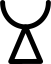
\includegraphics[height=0.4\textheight]{/home/tim/github/projects/../TART/doc/img/antenna.jpg}
  \end{center}
  \end{column}
  \begin{column}{0.6\linewidth}
   \includegraphics[width=\textwidth]{../top_view.jpg}
  \end{column}
  
 \end{columns}
\end{frame}

 \begin{frame}{Telescope Electronics}
\centering
 \includegraphics[height=0.4\textheight]{/home/tim/github/projects/../TART/doc/img/control_board_photo.png}
 \includegraphics[height=0.4\textheight]{/home/tim/github/projects/../TART/doc/img/radio_hub_photo.jpg}

 \includegraphics[width=0.7\linewidth]{/home/tim/github/projects/../TART/doc/img/radio_module.png}
\end{frame}



\begin{frame}
 \includegraphics[width=\linewidth]{fig/browser_view.jpg}
\end{frame}

\section{Synthesis Imaging}


\begin{frame}{Synthesis Imaging}
Measure complex visibility $V_{ij}$ by correlating signals from antenna $i$ and $j$.
\[ V_{ij} = \frac{1}{T} \int_0^T E_i(t) E_j^{\star}(t) dt \]
\begin{columns}
 \begin{column}{0.55\linewidth}
\begin{enumerate}
 \item 276 Pairs of antennas
 \item 16.368 MHz sampling rate per antenna
 \item Real-time correlation in FPGA
 \item 4.5 Giga MAC per second
 \item T $\sim$ 1 second
\end{enumerate}
 \end{column}
 \begin{column}{0.45\linewidth}
 \includegraphics[width=\linewidth]{fig/papilio_pro.jpg}
 \end{column}
\end{columns}

\end{frame}

\begin{frame}{Synthesis Continued...}
Fourier transform relationship between radio sky brightness $I(l,m)$ and
visibility $V(u,v)$,
\[
  V(u,v) = \int I(l,m) e^{2\pi j(lu  + mv)} dl dm
\]
Obtain $I(l,m)$ through inverse Fourier transform of $V(u,v)$, 
\[
 I(l,m) = \mathscr{F}^{-1}\{V(u,v)\}
\]
where $V(u,v)$ is the visibility function sampled in the $uv$-plane at the locations of each antenna $(u_{ij},v_{ij})$ pair. 
\end{frame}


\begin{frame}{The Dirty Image}
For the TART telescope there are 24 antennas, 
and 276 antenna pairs
\begin{columns}
 \begin{column}{0.5\textwidth}
 \begin{figure}
\includegraphics[width=\linewidth]{/home/tim/github/projects/max/phd/talk/nzip/pdf/uv_plane_init.pdf}
\caption{U-V antenna pairs}
 \end{figure}
 \end{column}
 \begin{column}{0.5\textwidth}
 \begin{figure}
 \includegraphics[width=\linewidth]{/home/tim/github/projects/../molteno/physics/spotless/doc/beam_2017_10_21_19_38_39_UTC.png}
% \includegraphics[width=\linewidth]{/home/tim/github/projects/max/phd/talk/nzip/pdf/dirty_beam_power_init.pdf}  
\caption{Inverse Fourier Transform}
 \end{figure}
 \end{column}
\end{columns}

\end{frame}


\begin{frame}{Swithing it on: Uncalibrated Image}
\begin{figure}
\includegraphics[height=0.9\textheight]{../uncalibrated_2017_10_21_19_38_39_UTC.png} 
\end{figure}
\end{frame}


\section{Calibration}

\frame{\tableofcontents[currentsection]}

\begin{frame}{Visiblity Calibration}
Define observed visibility between antennas $i$ and $j$ as
\[ \widetilde{V}_{ij} = G_{ij} V_{ij} + \epsilon_{ij} + \eta_{ij} \]
\begin{itemize}
 \item $G_{ij}$ is the complex gain, 
 \item $V_{ij}$ the true visibility, 
 \item $\epsilon_{ij}$ an additive error, and $\eta_{ij}$ is a noise term.
\end{itemize}
Convert $G_{ij}$ into antenna-based calibration quantities
\[ {G}_{ij} = g_{i}(t) g^{*}_{j}(t) = A_i(t)A_j(t) e^{j(\phi_i(t)-\phi_j(t))} \]
Where $g_i(t) = A_i(t) e^{j \phi_i(t)}$ is the {\bf complex gain} of the $i$th antenna.
\end{frame}

\begin{frame}{Calibration Parameters}
\centering
 \begin{tabular}{l|c|c|r}
  Description & Symbol & Units & $n$ \\ 
  \hline 
  Antenna Positions & $(x_i,y_i)$ & m & 48 \\
  Global Rotation Angle & $\Theta_0$ & \degree & 1 \\
  Receiver Gain & $A_i$ &  & 24 \\
  Receiver Phase Offset & $\phi_i$ & \degree & 24 
 \end{tabular}
\end{frame}


\begin{frame}{Easy Calibration: Antenna Positions}
\begin{columns}
 \begin{column}{0.5\linewidth}
\includegraphics[width=\linewidth]{/home/tim/github/projects/max/phd/talk/nzip/pdf/ant_pos.pdf}
  \end{column}
 \begin{column}{0.5\linewidth}
  Surveying problem:
  \begin{itemize}
   \item 3 Reference posts
   \item Measure distances to antennas
   \item Least-Squares minimize to get positions
   \item Residuals $< 2.5$mm
  \end{itemize}
  \begin{block}{Note}
Global rotation $\Theta_0$ still not accurate   
  \end{block}
 \end{column}
\end{columns}
\end{frame}

% \begin{frame}{CLEAN: H\"ogbom 1974}
% \begin{columns}
%  \begin{column}{0.5\linewidth}
% %  \includegraphics[width=\linewidth]{2017_10_21_19_38_39_UTC_uvfits_difmap.png}
%   \end{column}
%  \begin{column}{0.5\linewidth}
%   Image is the sum of point sources and a residual
%   \begin{eqnarray*}
%  I(l,m) & = & A_0 \delta(l_0, m_0) + I_0(l,m) \\
%  I_0(l,m)  & = & A_1 \delta(l_1, m_1) + I_1(l,m) \\
% 	   & = & \ldots
%   \end{eqnarray*}
%  \end{column}
% \end{columns}
% \end{frame}

\subsection{Satellites as Guide Stars}

\begin{frame}{The Guide Stars}
 \begin{columns}
  \begin{column}{0.5\linewidth}
   \includegraphics[height=0.9\textheight]{fig/QZS-1.jpg}
  \end{column}
  \begin{column}{0.5\linewidth}
  \begin{itemize}
   \item Position known to millimeters
   \item $>20000$ km away (point sources)
   \item Signal is `noise-like'
  \end{itemize}
   \includegraphics[width=\textwidth]{fig/qzss_ground_track.jpg}
   {\tiny Image: JAXA}
  \end{column}
 \end{columns}
\end{frame}

\begin{frame}{Calibration Data}
JSON files from the telescope API server
\begin{itemize}
 \item Visibility data (276 complex numbers per observation)
 \item Elevation and azimuth of known sources.
\end{itemize}
Typically 3 observations separated by 20 minutes.
\end{frame}


\subsection{Optimization Criterion}

\begin{frame}{Optimization Parameters}
\begin{center}
 \begin{tabular}{l|c|c|r}
  Description & Symbol & Units & $n$ \\ 
  \hline 
  Antenna Locations & $(x_i,y_i)$ & m & 48 \\
  Global Rotation Angle & $\Theta_0$ & \degree & 1 \\
  Receiver Gain & $A_i$ &  & 24 \\
  Receiver Phase Offset & $\phi_i$ & \degree & 24 
 \end{tabular}
\end{center}
 Remaining calibration parameters are make a 47-element vector
\[ \mathbf{x} = (\Theta_0, \Re(g_i), \Im(g_i)) \]
where $\Re(g_i)$ and $\Im(g_i)$ are the real and imaginary parts of the $i$th complex gain for the $i$th antenna
\begin{block}{Why not 49 parameters?}
Assume $g_0 = 1 + 0j$ as gains and phases are relative.
\end{block}
\end{frame}

\begin{frame}{Optimization Function}

Combines known-source intensity, and signal-to-noise ratio:
\[ -f(\mathbf{x}) = S(\mathbf{x}) + \sum_{j=1}^{N_s} K(l_j,m_j), \]
where:
\begin{itemize}
 \item $S(\mathbf{x})$ is the signal-to-noise ratio of the image $I(l,m)$ synthesized from the measured visibilities assuming the calibration parameters $\mathbf{x}$, 
 \item $K(l_j,m_j)$ is the intensity at the position of the $j$-th known source in the image $l,m$ plane, 
 \item $N_s$ is the number of known sources.
\end{itemize}

\end{frame}

The calibration procedure optimizes $f(\mathbf{x})$ over the space of possible calibration parameters. This
has 49 dimensions, although two of them are fixed to as phases and amplitudes are relative. This leaves 47 parameters to be determined from $246 \times M$ visibility measurements, 


\subsection{Basin Hopping}

\begin{frame}{Basin Hopping}
Offspring of a Metropolis-Hastings and a Steepest Descent Optimizer.
\begin{enumerate}
 \item Local-Minima using Quasi-Newton method
 \item `Hops' randomly to new part of parameter space
 \item Accept/Reject based on a Metropolis Criterion
\end{enumerate}
\begin{center}
\includegraphics[width=0.7\linewidth]{fig/basin_hopping.jpg} \\ {\tiny Image: Hashima et al}
\end{center}
% Developed to find minimum-energy configurations of complex molecules (with hundreds of degrees of freedom).
% The algorithm we use for the nonlinear optimization is Basin-Hopping. Basin-hopping~\cite{li1987monte, wales1997global, zhan2004multicanonical} is a stochastic algorithm that 
% combines a Monte-Carlo method with a steepest descent minimization. 
% The algorithm finds local minima using a Quasi-Newton method, and then `hops' to a new part of parameter space using random perturbations of co-ordinates. At each `hop' the
% new minimum is accepted or rejected using a Metropolis criterion. If $\Delta E$ is the difference between current minimum and the lowest known minimum, then if $\Delta E < 0$,
% the new minimum is always accepted. If $\Delta E$ is positive, then it is accepted with probability $e^{\Delta E}{T}$ where $T$ is the 'temperature', a tuning parameter for the
% optimizer.


\end{frame}
\section{Results}

\frame{\tableofcontents[currentsection]}


\begin{frame}
  \includegraphics[width=\linewidth]{../BH/bh_cost_history.pdf}
\end{frame}


\begin{frame}{Results}
\includegraphics[width=0.5\textwidth]{../uncalibrated_2017_10_21_19_38_39_UTC.png}\includegraphics[width=0.5\textwidth]{../calibrated_2017_10_21_19_38_39_UTC.png}
\end{frame}


% \begin{frame}{Calibrated Dirty Image}
% \includegraphics[height=0.9\textheight]{../calibrated_2017_10_21_19_38_39_UTC.png}
% Calibrated dirty image from the TART telescope. Known sources are circled. This shows a much 
% higher signal-to-noise ratio, as well as good agreement between peaks and known sources.
% \end{frame}

\begin{frame}{Calibrated Clean Image}
\begin{center}
\includegraphics[height=0.9\textheight]{../tart_clean.png}
\end{center}
\end{frame}
% Final clean image from the calibrated TART telescope. This image has a phase-center at 90 degrees elevation, and encompasses the sky in all directions to the horizon.


\begin{frame}
\begin{figure}[h!]
\centering    
\movie[label=show3,width=0.8\textwidth,poster,autostart,showcontrols,loop] 
   {\includegraphics[width=0.8\textwidth]{fig/spotless_2017_11_03_05_45_08_UTC.png}}{fig/spot_gridless.mp4}
  \caption{Point-Source Deconvolution (CLEAN) from TART data}
 \end{figure} 
\end{frame}



\section{Antenna Calibration from C/A}

\frame{\tableofcontents[currentsection]}

% \begin{frame}{Object Tracking}
% \centering    
% \movie[label=show4,width=\textwidth,poster,autostart,loop] 
%    {\includegraphics[width=0.6\textwidth]{fig/vlcsnap-2017-12-03-23h02m16s863.jpg}}{fig/unknown_object.mp4}
% 
% \end{frame}

\begin{frame}{Antenna Calibration}
\includegraphics[width=\linewidth]{../postgresinput_map_5_nside_6_orth.pdf}
\end{frame}


\begin{frame}{Orbit Determination}
\begin{columns}
\begin{column}{0.4\linewidth}
   \begin{itemize}
    \item Angles-Only Measurements
    \item Large Uncertainty $\sim 2 \degree$
    \item 6 Unknown Orbital Parameters
   \end{itemize}
\end{column}
\begin{column}{0.6\linewidth}
 \includegraphics[width=\linewidth]{fig/el_plot.pdf}
\end{column}
\end{columns}
 
\end{frame}


%  
%  \begin{frame}{Gridless}
%   \[ 
%    I(\theta,\phi) = \sum V_{i,j,k} e^{2 \pi i(u_i l + v_j m + (n-1) w_k )}
%   \]
% \begin{columns}
%  \begin{column}{0.5\linewidth}
%   \begin{eqnarray*}
%    l & = & \sin(\phi) \cos(\theta) \\
%     m & = & \cos(\phi) \cos(\theta) \\
%     n & = & \sin(\theta) 
%   \end{eqnarray*}
%   \begin{itemize}
%    \item $\theta, \phi$ are elevation and azimuth
%    \item $n$ often written in this weird way... $n = \sqrt{1 - l^2 - m^2}$
%    \item  Can be evaluated directly (no FFT or IFFT)
%   \end{itemize}
%  \end{column}
%  \begin{column}{0.5\linewidth}
%  \includegraphics[width=\linewidth]{gridless_2017_10_21_19_38_39_UTC.png}
%  \end{column}
% \end{columns}
% \end{frame}
% 
% 
% \begin{frame}{Gridless: Advantages}
%  \begin{itemize}
%   \item Direct Fourier Transform (rather than the FFT).
%   \item No Gridding
%   \item Slower (for many vis)
%   \item Can be trivially parallelized
%   \item Image is calculated in $(\theta,\phi)$
%   \item Full-Sky and no w-projection needed
%   \item healpix
%  \end{itemize}
% 
% \end{frame}

% \section{Spotless}
% 
% \begin{frame}{Spotless}
%   \begin{eqnarray*}
%   V(u,v,w) & = & A_0 V_P(\theta_0, \phi_0) + V_0(u,v,w) \\
%   V_0(u,v,w) & = & A_1 V_P(\theta_1, \phi_1) + V_1(u,v,w)
%  \end{eqnarray*}
% \begin{columns}
%  \begin{column}{0.5\linewidth}
%   \begin{eqnarray*}
%    A_0 & = & \min_{A, \theta, \phi} E(V_0) \\
%        & = & \min_{A, \theta, \phi} E(V - A V_P(\theta, \phi))
%  \end{eqnarray*}
%   \begin{enumerate}
%    \item $V_P(\theta, \phi)$ is the forward map
%    \item $V_i(u,v,w)$ is the residual
%    \item Visibilities from a point source located at $(\theta, \phi)$ with intensity $A$.
%   \end{enumerate}
%  \end{column}
%  \begin{column}{0.5\linewidth}
% %  \includegraphics[width=\linewidth]{spotless_2017_10_21_19_38_39_UTC.png}
%  \end{column}
% \end{columns}
% \end{frame}
% 
% 
% \begin{frame}{Parseval's theorem}
%    \[ \int d\theta \int d \phi I(\theta, \phi)^2 =  \int du \int dv |V(u,v)|^2 \]
% \begin{enumerate}
%  \item Energy in image $E(I) = \int I(\theta, \phi)$
%  \item Energy in image $E(V) = \sum_{i,j} |V_ij|^2$
%  \item Can be evaluated directly in visibility space
%  \item $O(N^2)$ where $N$ is the number of antennas
%  \item So minimization of residual energy is possible without FFT or IFFT
% \end{enumerate}
% \end{frame}
% 
% 
% \begin{frame}{Spotless: Generating the model}
%  
%  \begin{itemize}
%   \item Initial Guess by brute force 
%   \item Minimize the residual energy to get point properties
%   \item Repeat.
%  \end{itemize}
% 
% \end{frame}

% \begin{frame}{Residual}
% \begin{columns}
%  \begin{column}{0.5\linewidth}
%  Lots of noise
%  \end{column}
%  \begin{column}{0.5\linewidth}
%  \includegraphics[width=\linewidth]{residual_2017_10_21_19_38_39_UTC.png}
%  \end{column}
% \end{columns}
% \end{frame}
% 
% 
%  \begin{frame}{Restored Image}
% \begin{columns}
%  \begin{column}{0.5\linewidth}
%  \includegraphics[width=\linewidth]{2017_10_21_19_38_39_UTC_uvfits_difmap.png}
%  \end{column}
%  \begin{column}{0.5\linewidth}
%  \includegraphics[width=\linewidth]{spotless_2017_10_21_19_38_39_UTC.png}
%  \end{column}
% \end{columns}
% \end{frame}



\begin{frame}{What the future holds}
\begin{itemize}
 \item Automatic Tracking
 \item New Imaging Algorithms (Gridless, Direct from Data)
 \item TART 2.5. Zync 7020.
 \item TART 3.0. 96-Antennas! 400m baselines.
 \item Transient Event Detection
 \item South Africa (Stellenbosch) now online
\end{itemize}
\includegraphics[width=\linewidth]{fig/alma.jpg}
 
\end{frame}

\begin{frame}
\includegraphics[width=\linewidth]{fig/radio_agronomy.jpg}
\end{frame}


\end{document}
